\section{Experimental Setup \label{sec:setup}}
\subsection{Platform and Models\label{sec:platform}}
%Describe hardware
\cparagraph{Hardware.} Our experimental platform is a NVIDIA Jetson TX2 embedded platform. The system has a 64~bit dual-core Denver2 and a
64~bit quad-core ARM Cortex-A57 running at 2.0~Ghz, and a 256-core NVIDIA Pascal GPU running at 1.3~Ghz. The board has 8~GB of LPDDR4 RAM
and 96~GB of storage (32~GB eMMC plus 64~GB SD card).


%Describe software
\cparagraph{System Software.} We run the Ubuntu 16.04 operating system with Linux kernel v4.4.15. We use Tensorflow v.1.6, cuDNN (v6.0) and
CUDA (v8.0.64).


\cparagraph{Deep Learning Models.} We consider 11 pre-trained \CNN models for image recognition from the TensorFlow-Slim library~\cite{silberman2013tensorflow} and a recurrent neural network (\RNN) model for machine translation. Table~\ref{tbl:workload} lists the models considered in this work.



\begin{table}[t!]
\begin{center}
\vspace{-1mm}
\caption{Considered workloads and the statistical information
 on the non-blacklist subset of the validation set of ILSVRC 2012 and WMT 2016}
\vspace{-2mm}
\scriptsize
\label{tbl:workload}
\begin{tabular}{llllll}
\toprule
\textbf{Model}&\textbf{Neuronal Style}& \textbf{Top-1} & \textbf{Top-5}& \textbf{Top-5}& \textbf{Layer Depth} \\
\midrule
\textbf{Mobilenet\_v1\_1.0} & Convolutional & 70.7 & 89.56 &	4.2M	&28 \\
\textbf{Inception\_v1}     &Convolutional & 69.8  & 89.6	&7M&	22  \\
\textbf{Inception\_v2}     &Convolutional &73.9	&91.4 & 11.3M& 	32 \\
\textbf{Inception\_v3}     &Convolutional  & 78	&94 &	27.1M	&42 \\
\textbf{Inception\_v4}     &Convolutional& 80.2	&95.2 & &58 \\
\textbf{ResNet\_50}        &Convolutional & 75.2&	90.2&	25.5M &	50\\
\textbf{ResNet\_101} &Convolutional &76.4	&92.9&	51M&	101  \\
\textbf{ResNet\_152} &Convolutional & 76.8	&93.2&	76.5M	&152\\
\textbf{VGG\_16} &Convolutional, Full & 71.5&	89.8	&138M	&16 \\
\textbf{VGG\_19} &Convolutional, Full & 71.1	&89.8	&138M	&19  \\
\textbf{NMT} &Recurrent  & 27.4(BLEU)	& -	&211M	&4 \\
\bottomrule
\end{tabular}
\end{center}
\vspace{-6mm}
\end{table}


\begin{figure*}[!t]
\centering
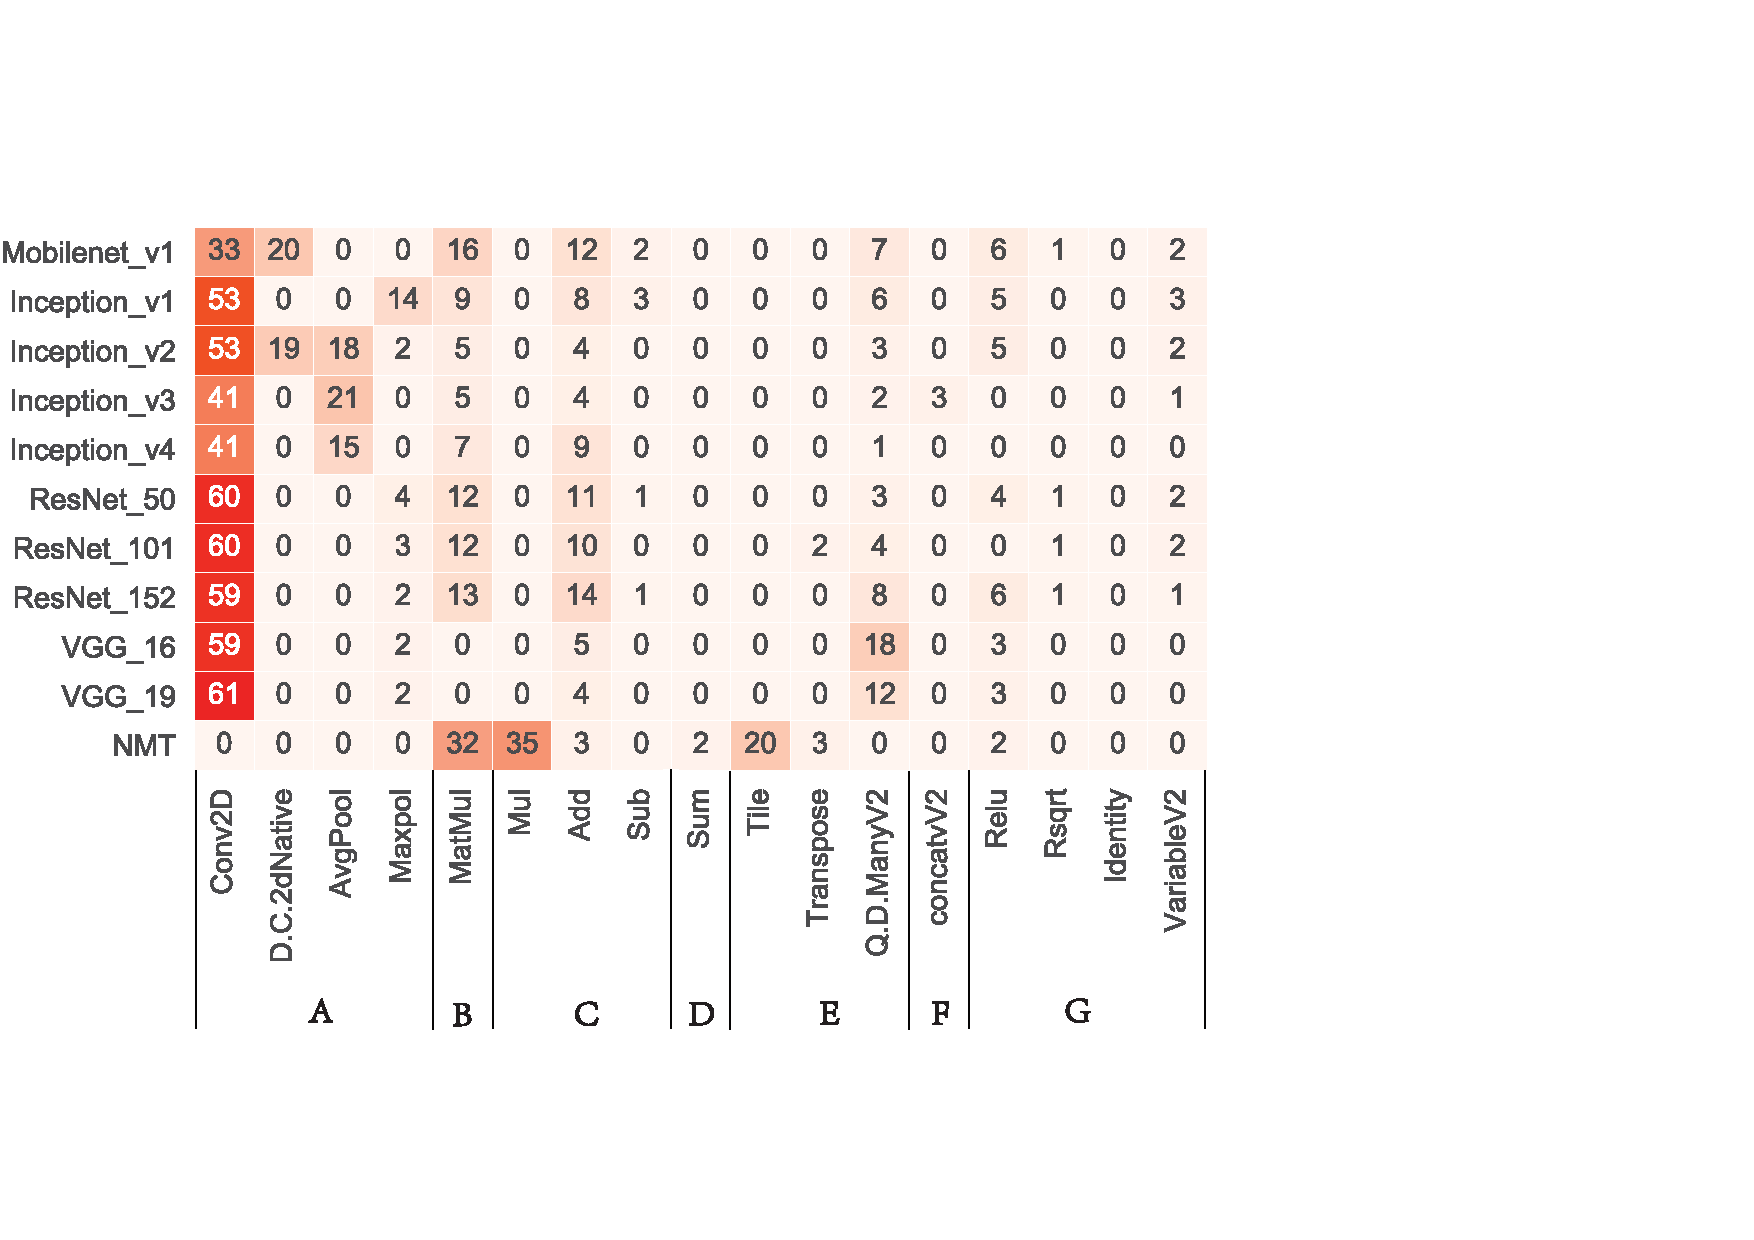
\includegraphics[width=0.7\textwidth]{figure/break11models.pdf}
\caption{ Breakdown of execution time by operation type for every listed models in Table~\ref{tbl:workload}.\\
(D.C.2dNative: DepthwiseConv2dNative, Q.D.ManyV2: QueueDequeueManyV2, V.V2: VariableV2)}
 \label{fig:breakdown11}

\end{figure*}
 %The models are built using TensorFlow and trained on the ImageNet ILSVRC 2012 training set.


\subsection{Evaluation Methodology \label{sec:method}}

\cparagraph{Performance Metrics} We consider the following metrics:
%\vspace{-2mm}
\begin{itemize}
\item \emph{\textbf{Inference time} (lower is better)}. Wall clock time between a model taking in an input and producing an output,
    excluding the model load time.

\item \emph{\textbf{Energy consumption} (lower is better)}. The energy used by a model for inference.  We deduct the static power used by
    the hardware when the system is idle.

\item \emph{\textbf{Accuracy} (higher is better)}. The ratio of correctly labeled images to the total number of testing instances.

\item \emph{\textbf{Precision} (higher is better)}. The ratio of a correctly predicted instances to the total number of instances that
    are predicted to have a specific label. This metric answers e.g., ``\emph{Of all the images that are labeled to have a cat, how many
    actually have a cat?}".

\item \emph{\textbf{Recall} (higher is better)}. The ratio of correctly predicted instances to the total number of test instances that
    belong to an object class. This metric answers e.g., ``\emph{Of all the test images that have a cat, how many are actually labeled to
    have a cat?}".

\item \emph{\textbf{F1 score} (higher is better)}.  The weighted average of Precision and Recall, calculated as $2\times\frac{Recall
    \times Precision} {Recall + Precision}$. It is useful when the test dataset has an uneven distribution of classes.

\item \emph{\textbf{BLEU} (higher is better)}. The bilingual evaluation understudy (BLEU) evaluates the quality of machine translation.
    The quality is considered to be the correspondence between a machine's output and that of a human: ``\emph{the closer a machine
    translation is to a professional human translation, the better it is}". We report the BLUE value on \texttt{NMT}, a machine
    translation model.


\end{itemize}

\cparagraph{Performance Report.}   For image recognition, the accuracy of a model is evaluated using the top-1 score by default; and we
also consider the top-5 score. We use the definitions given by the ImageNet Challenge. Specifically, for the top-1 score, we check if the
top output label matches the ground truth label of the primary object; and for the top-5 score, we check if the ground truth label of the
primary object is in the top 5 of the output labels for each given model. For NLP, we use the aforementioned BLEU metric. Furthermore, to
collect inference time and energy consumption, we run each model on each input repeatedly until the 95\% confidence bound per model per
input is smaller than 5\%. In the experiments, we exclude the loading time of the \CNN models as they only need to be loaded once in
practice. To measure energy consumption, we developed a lightweight runtime to take readings from the on-board energy sensors at a
frequency of 1,000 samples per second. We then matched the energy readings against the time stamps of model execution to calculate the
energy consumption.
